\documentclass[conference]{IEEEtran}
\IEEEoverridecommandlockouts
% The preceding line is only needed to identify funding in the first footnote. If that is unneeded, please comment it out.
\usepackage{cite}
\usepackage{amsmath,amssymb,amsfonts}
\usepackage{algorithmic}
\usepackage{graphicx}
\usepackage{textcomp}
\usepackage{xcolor}
\usepackage{float}

\usepackage[utf8]{inputenc}
\usepackage[english]{babel}
\usepackage{fancyhdr}
\usepackage{lastpage}
\pagestyle{fancy}
\fancyhf{}
 
\rfoot{\thepage}

\def\BibTeX{{\rm B\kern-.05em{\sc i\kern-.025em b}\kern-.08em
    T\kern-.1667em\lower.7ex\hbox{E}\kern-.125emX}}
\begin{document}

\title{Brain Tumor Detection}

\author{\IEEEauthorblockN{1\textsuperscript{st} Luís Silva}
\IEEEauthorblockA{\textit{DETI} \\
\textit{Universidade de Aveiro}\\
Aveiro, Portugal \\
NMEC: 88888}
\and
\IEEEauthorblockN{2\textsuperscript{nd} Pedro Amaral}
\IEEEauthorblockA{\textit{DETI} \\
\textit{Universidade de Aveiro}\\
Aveiro, Portugal \\
NMEC: 93283}
\and
\IEEEauthorblockN{3\textsuperscript{rd} Pedro Tavares}
\IEEEauthorblockA{\textit{DETI} \\
\textit{Universidade de Aveiro}\\
Aveiro, Portugal \\
NMEC: 93103}
}

\maketitle

\begin{abstract}
Brain tumor detection is a process performed every day by specialized doctors. Yet, it is also a classification problem whose objective is to analyze the presence or absence of tumors in the brain through various imaging techniques. This detection is crucial for the patient because if the tumor is detected in its early stages, the survival rate rises tremendously and with fewer complications throughout the treatment process. To develop our solution, a data set with 253 images from MRI scans of the human brain.
\end{abstract}

\begin{IEEEkeywords}
brain, tumor, CNN, convolution, SVG, Transfer learning
\end{IEEEkeywords}

\section{Introduction}
Brain tumor detection is a useful process in the real world, mainly in edge cases where it is hard to determine if the tumor exists or not. This is true because, the earlier the tumor gets detected, the sooner it can be treated, leading to an easier and higher chance of survival for the patient.

This report contains 3 models which attempt to solve this problem using different machine learning approaches. In the next sections, we will first start by analyzing existing work regarding this theme Then the techniques associated with processing the data set will be explained. Next, the model's architecture will be detailed and the selection of its hyper-parameters will be described. Finally, a comparison will be made between the different models implemented.

This project was made in the context of the machine learning course at the University of Aveiro under the teacher Pétia Georgieva. 


\section{State of the Art\cite{b4}\cite{b5}\cite{b8}}

When starting a project in machine learning it is always important to analyze previous work related to the theme of the data set. Most of the time, other people have already worked on similar data sets or even in the same data set. Given that our data set is from Kaggle there were a lot of projects that we could easily access about it.

Most of the previous work in this data set and theme used transfer learning which uses previously trained models to create another, using mostly VGG16 but also ResNet50. Besides transfer learning, convolutional neural networks are also very used in this theme since they are the most used for images in general. Outside of deep learning, Support Vector Machine is the most popular algorithm. Given this research, we decided that these would be the 3 models that would be implemented in this project.

Another factor apparent from our research is that most existing projects try to achieve better results using data augmentation to increase the size of the data set by artificially creating more examples.

\section{Data Set Analysis}
To train the models present in this project, a data set from Kaggle containing 253 images containing brain magnetic resonance images classified into 2 classes: positive and negative. In the images below we can see some examples from the used data set.

\begin{figure}[H]
    \centering
    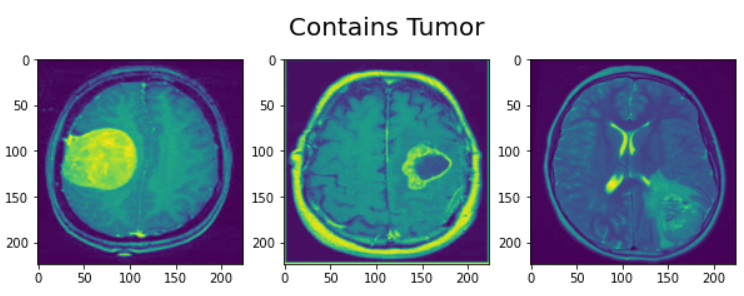
\includegraphics[width=3.5in]{has_tumor.PNG}
    \caption{Examples of MRI with tumor}\label{fig:fig1}
\end{figure}

\begin{figure}[H]
    \centering
    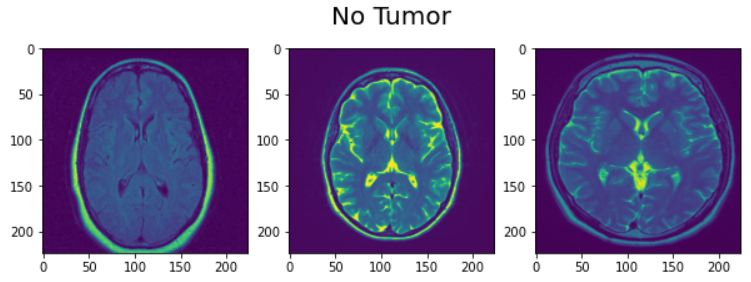
\includegraphics[width=3.5in]{hasnt_tumor.PNG}
    \caption{Examples of MRI without tumor}\label{fig:fig2}
\end{figure}

From these, we can observe that there are several differences between examples from the same class but there are certain details that are common that our algorithm should be able to distinguish. Our data set also presents a slight imbalance in the distribution of images between both classes.

\begin{figure}[H]
    \centering
    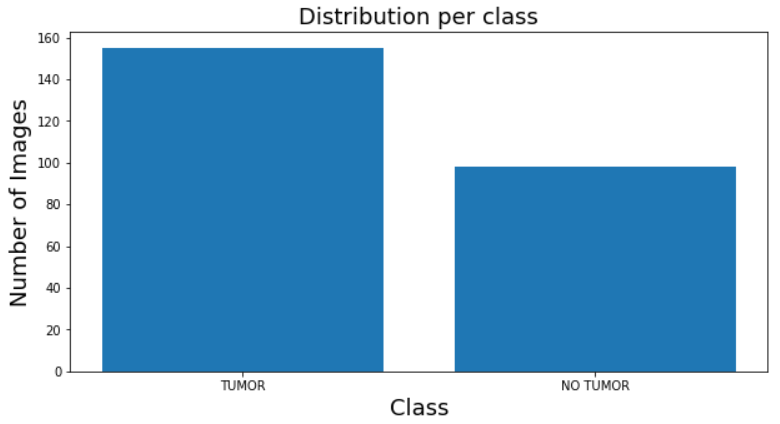
\includegraphics[width=3.5in]{class_distribution.PNG}
    \caption{Distribution of images between the classes}\label{fig:fig3}
\end{figure}

Given this imbalance, data set balancing methods such as oversampling (repeat example from the smallest class) and undersampling (ignore examples from the largest class) may be beneficial.
Besides the imbalance of classes, the data set used is small which may lead to some consistency problems. Since the amount of data is small, when compared to most data sets, the models will have fewer examples to train from. This problem could be solved through the use of data augmentation, which is a form of creating artificial data through the original data set and adding variety. This augmented data can be used as the training set used to train the model which should benefit the model by having more, and more varied data to pick from when training.

\section{Data Pre-processing}

Before we use our data set in the models, its data must be prepared in a way that increases the performance of our algorithms. Given that we have different models, not every model used every single one of the implemented techniques using only the ones that made that model more effective.

\subsection{Gray-scale Transformation}

Our data set contains brain magnetic resonance images which are artificially given colors. This makes the color irrelevant for this project and therefore, When the images are read, they are always read in grayscale.

\subsection{Cropping}

Another technique that was used was cropping the image so that only the essential parts are left. This makes it so that when a future resizing happens less relevant information is lost. Despite this, the only model that seemed to benefit from cropping was the Convolutional Model giving the other 2 equal ao inferior performances when used.

\subsection{Resizing}

Resizing was another technique that was used in every model since, for the model to be trained, all the images given to him must have the same size.

\subsection{Normalizing}

Normalizing consists of converting every pixel to a value between 0 and 1 so that it becomes easier for the model to learn from the data. Despite this, it was not used in the Transfer Learning Model since it severely reduced its performance.

\subsection{Shuffling}

Finally, the data was also shuffled so that the model can learn more effectively from our data set. This is another mandatory step and therefore it happened in the preprocessing for every model.

\section{Implemented Models}

\subsection{SVM Model}
Support Vector Machine is a supervised learning model, it's goal is to separate the classes by defining a hyperplane through an N-dimensional space, with N being the number of features. Hyperplanes are essentially decision boundaries and while many could be drawn our goal is to choose the one that best fits our data while leaving room so that new, future data can be analyzed with confidence. This is achieved by choosing the one that maximizes the distance between two points of our classes.

Our implementation was based on the code presented in \cite{b10} and \cite{b11}.

\begin{figure}[H]
    \centering
    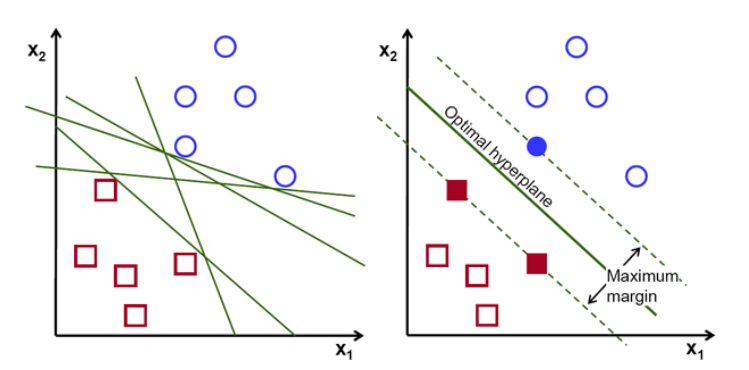
\includegraphics[width=3.5in]{SVM_margin.png}
    \caption{Maximization of margin when choosing a hyperplane}\label{fig:fig3}
\end{figure}

The support vectors that give name to the model are the points of each class that fall closer to the hyperplane, these influence the plane's position and orientation. Deleting or adding data points within the margin (before training) will result in a change to the resulting hyperplane.\\
The model can be tweaked by changing a few parameters\\

\subsubsection{C}

This parameter denotes the importance given to a misclassification of an example. The higher C is the higher the penalty. Increasing C will give more emphasis to fitting the curve to the training data which may lead to overfitting, decreasing C will put more emphasis on the generalization of the properties and thus can lead to a model that is better fitted to classify future examples.\\

\subsubsection{Gamma}
Determines how fast the similarity drops to 0 as elements get further apart, defines the influence of single training examples. Gamma is equal to \[1/2*\sigma^2, \sigma-variance\] with and lower gamma means higher bias/variance and higher gamma means lower variance/variance.\cite{b9}\\

\subsubsection{Kernels}
Set of mathematical functions that map lower-dimensional data into higher dimensional-data.\\

\subsection{CNN Model}
A convolutional neural network consists of a series of layers. The input layer, hidden layers that perform convolutions which are essentially a mix of two functions to generate a third one and the output layer.\\
 

\subsubsection{Architecture}
In our CNN model, we applied zero padding and defined the activation function as leaky ReLU, a version of ReLU, and two convolutional layers to process the images. The first one applies 64 filters and the second one, 128, both with a kernel size of 4x4 and strides of 1x1, after both convolutional layers, a max-pooling layer was added with a kernel size of 4x4 and the same dimension for the corresponding strides. After the first max-pooling a dropout layer was added to ignore 30\%of the data at random whose main objective is to prevent overfitting. After all that is done, the data is flattened and goes through two dense layers, the first being of the type ReLU and the second of type sigmoid. Finally, it is compiled using Adam's optimizer and the SparseCategoricalCrossEntropy.
Having this in consideration, the data processing sequence is as follows:
\begin{figure}[H]
    \centering
    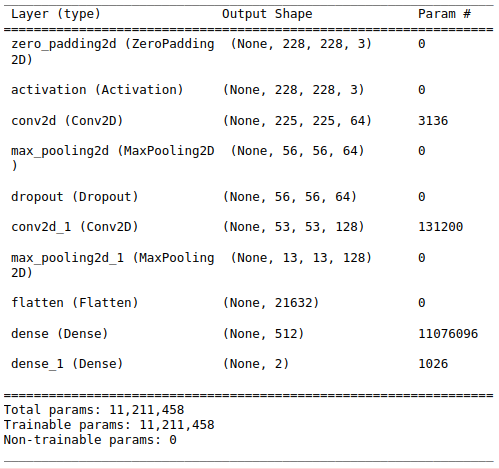
\includegraphics[width=3.5in]{CNN-Architecture.png}
    \caption{CNN Model Parameters}\label{fig:fig4}
\end{figure}
    The first convolutional 2D layer has 36, the second has 64 and finally, the third one has 128 filters of size 4x4 with a horizontal and vertical stride of 1 pixel. Batch Normalization is made only once along with the results from the 36 filters applied in the first convolutional layer;
  Max Pooling of 4x4 pools, with horizontal and vertical strides of 4 pixels;
  Dropout Layer: ignores data and does this by setting to 0 20\% of the values of the input at random;
  
  Convolutional 2D layer with 64 filters of size 4x4 with a horizontal and vertical stride of 1 pixel.
  Max Pooling of 4x4 pools, with horizontal and vertical strides of 4 pixels;
  Dropout Layer: ignores data and does this by setting to 0 30\% of the values of the input at random;
  
  Convolutional 2D layer with 128 filters of size 4x4 with a horizontal and vertical stride of 1 pixel.
  Max Pooling of 4x4 pools, with horizontal and vertical strides of 4 pixels;
  
  Flatten to turn all the data into a 1D data structure;
  Dense with sigmoid activation;

\subsubsection{Activation Function}
For the activation function, in the CNN, we used a ReLU, which stands for Rectified Linear Unit which takes the input and if it is positive, it keeps it, otherwise, it sets its value to zero.\\

\subsubsection{Loss Function}
To determine if the predicted values are close to the real ones, there is a need to represent that discrepancy. To represent that discrepancy we are using the binary cross-entropy method which is one of the most commonly used in machine learning.\\

\subsubsection{Optimizer}
In this model, we decided to use Adam as our optimizer given that, according to our research, it is the most used optimizer. It combines the advantages of two other optimizers (Adaptive Gradient Algorithm and Root Mean Square Propagation) and outperforms them, being more efficient and using relatively less memory.\cite{b6}\\

\subsection{Transfer Learning Model}

Recapitulating, from our research most of the existing work regarding this theme uses transfer learning which consists in using a model already trained with a different but related data set in our model, therefore, applying existing knowledge to a new problem. Among the existing trained models, most of the existing work used VGG16 so our Transfer Learning Model will also use it. Our implementation was based on a model from kaggle\cite{b3} although some changes were made.

\subsubsection{Architecture}
Building our model besides the VGG16, a global pooling layer to reduce the dimensionality of the VGG16's output, a dropout layer to ignore 20\% of previous weights, and 3 dense layers were also added.

\begin{figure}[H]
    \centering
    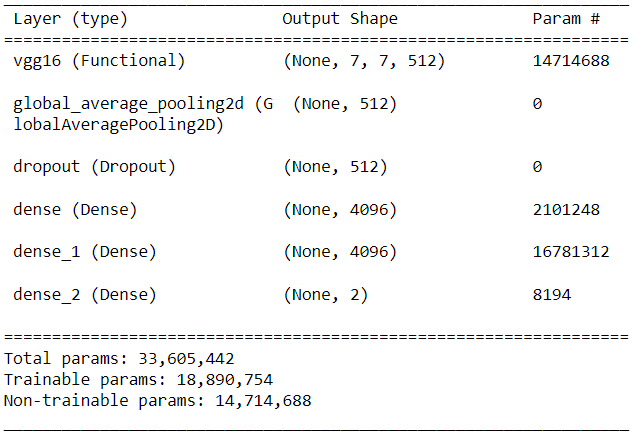
\includegraphics[width=3.5in]{transferl_model.PNG}
    \caption{Transfer Learning Model Parameters}\label{fig:fig5}
\end{figure}

\subsubsection{Activation Function}
In the dense layers added after VGG16, an activation function was needed. In the first 2, ReLU was used but in the final layer sigmoid was used which returns a value between 0 and 1 depending on the input.\\

\subsubsection{Loss Function}

In this model Sparse Categorical Cross-entropy was used which computes the cross-entropy loss between the real labels and predicted labels.\\

\subsubsection{Optimizer}
This model also uses the Adam optimizer like the previous model.

\section{Model Training}


To be able to correctly obtain and evaluate a model, our data set needs to be split into sets with different goals. Given that we had a sizable amount of examples compared to the number of classes we decided to use the standard way of splitting our data into Training Set (60\%), Validation Set (20\%), and Test Set (20\%).\cite{b7}\\

\subsubsection{Training Set}

This set has the biggest percentage of the original data set because this set will be used to train the model.\\

\subsubsection{Validation Set}

This set has the main function of testing our models across the iterations to validate our model's architecture and hyper-parameters during its development given that this data is not in the training set it is a good measure to see if our model is correctly generalizing and is not getting over-fitted. When the architecture and the hyper-parameters are decided they will be used to train the final model alongside the training set.\\

\subsubsection{Test Set}
This set contains data that the model has never seen in the development phase and neither in the final training and it is used to make a final evaluation of the implemented model.

\subsection{Data Augmentation}
Data augmentation is a method that allows generating a bigger amount of data from the original data set. This generation can be performed through a variety of transformations, in particular, random rotations, symmetry along horizontal and vertical axes, scaling, and brightness, among others. This method can be used for model training since it expands and increases the variety of the training set which, in theory, should make the model more flexible to slight changes to the real images. In our solutions, we used data augmentation in the SVM model. Data augmentation was tested in the CNN and Transfer Learning models as well, but the results were not as satisfactory as the model without data augmentation.

\subsection{Oversampling and Undersampling}

As previously referred to, our data set is imbalanced, and therefore an undersampling and an oversampling approach were used but the only positive result was applying oversampling in the SVM Model. The performance of the other 2 models was unaffected or decreased by these methods.

\subsection{Results}

Given the models and techniques described above, in this section, the results of the implemented algorithms will be detailed.

\subsubsection{SVM Model Validation}

Data augmentation is an interesting approach because our data set is small and because there is a noticeable discrepancy between the number of examples of class yes and class no as seen in fig. 7.

\begin{figure}[H]
    \centering
    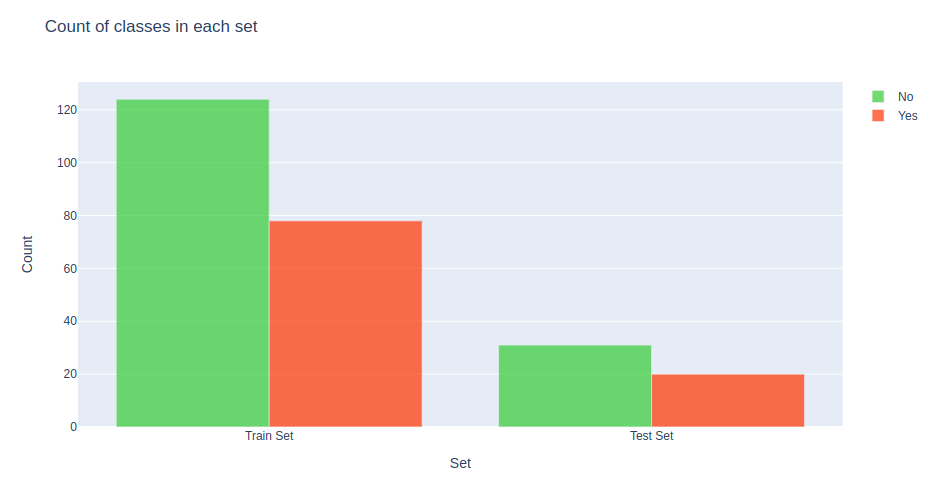
\includegraphics[width=3.5in]{SVM_classdistribution_begining.png}
    \caption{Class distribution in data sets without oversampling}\label{fig:fig6}
\end{figure}

Applying data augmentation and producing examples of class no and class yes at a rate of 2 to 1, not only provides more examples to train and validate our model but also balances out the classes' frequency, this is called oversampling. In fig.8 we can see the effect that this process had on our class distribution.

\begin{figure}[H]
    \centering
    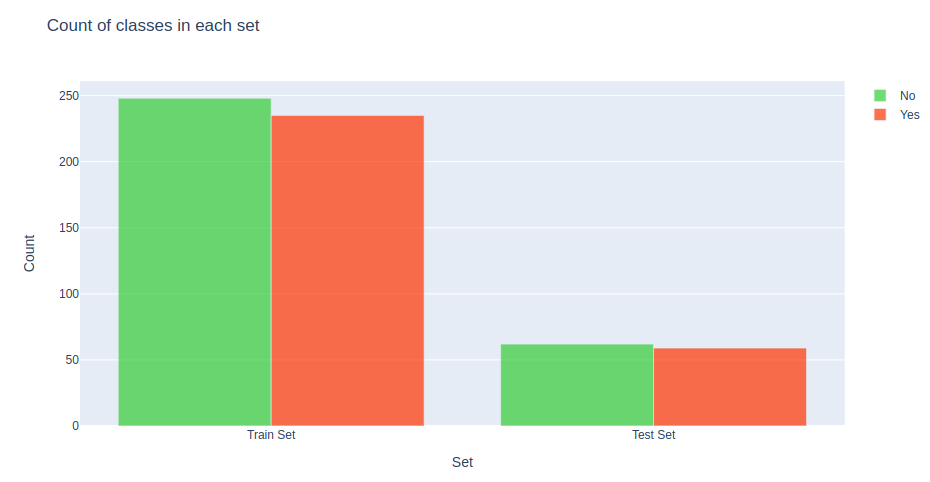
\includegraphics[width=3.5in]{SVM_classdistribution_oversamp.png}
    \caption{Class distribution in data sets with oversampling}\label{fig:fig7}
\end{figure}

Analyzing the confusion matrixes for the model, displayed in fig.9 and fig.10, we notice a drop in performance from classifying examples from the testing dataset to classifying examples from the validation dataset which is, although not desirable, expected as it is now dealing with examples it has never seen before.\\

\begin{figure}[H]
    \centering
    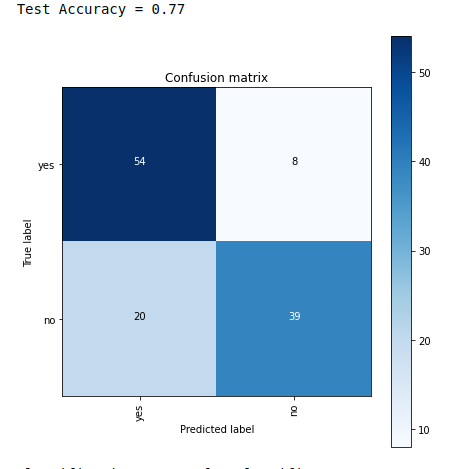
\includegraphics[width=3in]{SVM_final_accuracy.png}
    \caption{Accuracy in validation data set with oversampling}\label{fig:fig11}
\end{figure}

Table \ref{table:1} refers to the models evaluation.

\begin{table}[htbp]
\centering
\caption{Transfer Learning Model Statistics}
\begin{center}
\begin{tabular}{|c|c|}
\hline
Train Accuracy & 0.77 \\
\hline
Test Accuracy & 0.77 \\
\hline
Precision & 0.78\\
\hline
Recall & 0.77\\
\hline
F1 Score & 0.77 \\
\hline
\end{tabular}
\end{center}
\label{table:1}
\end{table}

\subsubsection{CNN Model Validation}\n
In the following images, we can see the evolution of the model training throughout all its epochs. And as we can see, the divergence between the training and validation set, both in accuracy and loss values are relatively similar, meaning that the model is capable of generalizing and is not overfitting.


\begin{figure}[H]
    \centering
    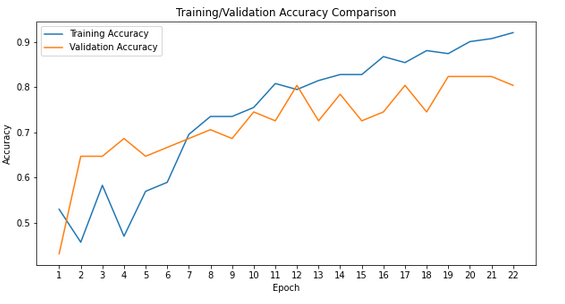
\includegraphics[width=3.5in]{cnn-epoch-accuracy.png}
    \caption{CNN Model Accuracy Comparison}\label{fig:fig12}
\end{figure}

\begin{figure}[H]
    \centering
    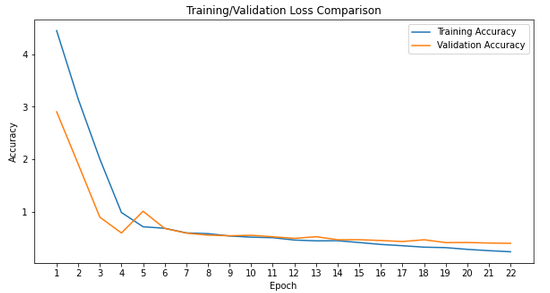
\includegraphics[width=3.5in]{cnn-epoch-loss.png}
    \caption{CNN Model Loss Comparison}
    \label{fig:fig13}
\end{figure}

When we look at the confusion matrix presented below we can understand that the probability of classifying correctly images that do not present a tumor is lower than the ones that present. A way to fix this issue would be to perform oversampling, yet it was not found that with this solution, the overall results, generally, were not as good as without the method being applied.

\begin{figure}[H]
    \centering
    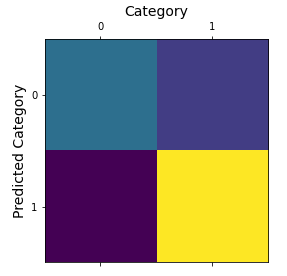
\includegraphics[width=3in]{cnn-confusion-matrix.png}
    \caption{Confusion Matrix of the CNN Model}\label{fig:fig6}
\end{figure}

\begin{table}[htbp]
\centering
\caption{CNN Model Statistics}
\begin{center}
\begin{tabular}{|c|c|}
\hline
Train Accuracy & 0.9007 \\
\hline
Validation Accuracy & 0.7255 \\
\hline
Test Accuracy & 0.8824 \\
\hline
Train Loss & 0.3005\\
\hline
Validation Loss & 0.7022 \\
\hline
Test Loss &  0.4898\\
\hline
Precision & 0.92\\
\hline
Recall & 0.88\\
\hline
F1 Score & 0.89 \\
\hline
\end{tabular}
\end{center}
\label{table:2}
\end{table}

\subsubsection{Transfer Learning Model Validation}

In the images below we can see the evolution of the accuracy and the loss throughout epochs during the validation of the optimized transfer learning model. Given that the graph from training and the one from validation are relatively close to one another we can conclude that the model did not suffer from over-fitting and can generalize.


\begin{figure}[H]
    \centering
    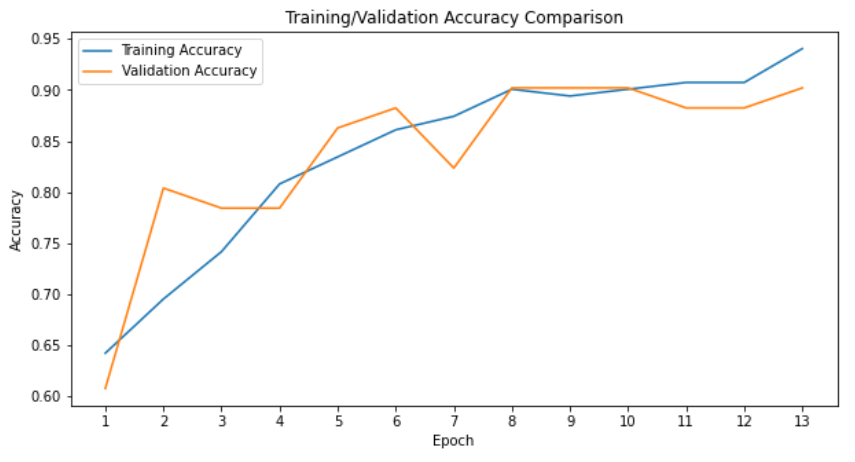
\includegraphics[width=3.5in]{transferl_val_accuracy.PNG}
    \caption{Transfer Learning Model Accuracy Comparison}\label{fig:fig14}
\end{figure}

In the table \ref{table:2} we can observe more statistics about the model.

\begin{figure}[H]
    \centering
    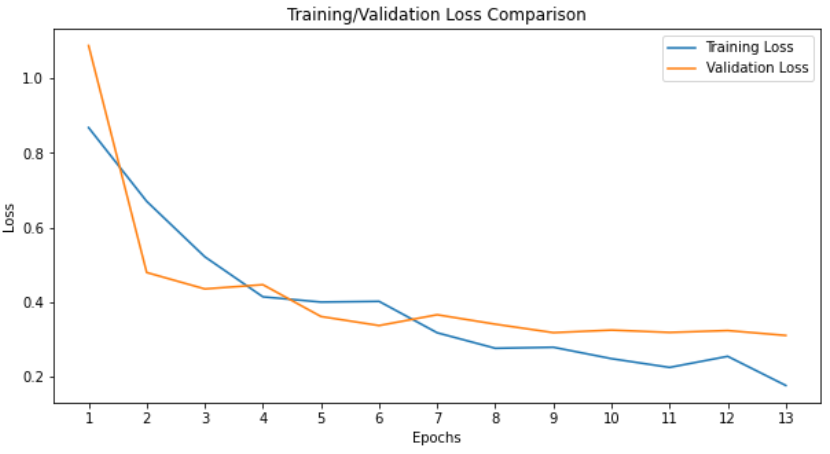
\includegraphics[width=3.5in]{transferl_val_loss.PNG}
    \caption{Transfer Learning Model Loss Comparison}\label{fig:fig15}
\end{figure}

From the confusion matrix below we can see that the model has a bigger probability of classifying an image as 1 (has tumor) than as a 0 (no tumor) and it also ends up classifying more 0s as 1s than the opposite. The major reason for this is the imbalance of classes in the data set but, as referred to at the beginning of the report, the attempts at fixing this by oversampling and undersampling ended up lowering the model performance as a whole.

\begin{figure}[H]
    \centering
    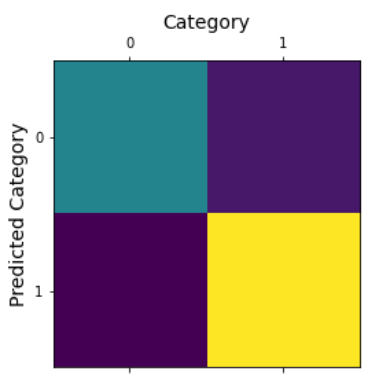
\includegraphics[width=3in]{tl_conf_matrix.PNG}
    \caption{Confusion Matrix of the Transfer Learning Model}\label{fig:fig6}
\end{figure}

In the table \ref{table:3} we can observe more statistics about the model.

\begin{table}[htbp]
\centering
\caption{Transfer Learning Model Statistics}
\begin{center}
\begin{tabular}{|c|c|}
\hline
Train Accuracy & 0.9216 \\
\hline
Validation Accuracy & 0.9020 \\
\hline
Test Accuracy & 0.9216 \\
\hline
Train Loss & 0.2470\\
\hline
Validation Loss & 0.3105 \\
\hline
Test Loss &  0.2470\\
\hline
Precision & 0.93\\
\hline
Recall & 0.92\\
\hline
F1 Score & 0.92 \\
\hline
\end{tabular}
\end{center}
\label{table:3}
\end{table}

\section{Hyper-Parameter Selection}

\subsection{SVM Model Hyper-Parameters}

\subsubsection{Grid Search}
The way that we are going to search for the best hyperparameters is through GridSearchCV. GridSearchCV is a function that receives a list of values for the C parameter, the Gamma parameter, and the kernel and trains all combinations of parameters to find the best one. For each combination, the function performs 5-fold cross-validation and iterates until convergence.\\

We entered as parameters for C the values 0.1, 1, 10, 100, for gamma the values 0.0001, 0.001, 0.1, 1 and kernel the options 'rbf','linear' and 'poly' and the combination with the best results was rbf with C=1 and gamma=0.0001.

\subsection{Number of Epochs}

The number of epochs is one of the most important hyper-parameters during the training phase of a deep learning model. It represents the number of times that the training data set will be seen by the model and therefore the number of times the model will try to adapt itself to the input data. If it is chosen incorrectly it can result in under-fitting which means that the model will not be able to correctly detect the relevant features or over-fitting where the model is unable to generalize beyond the training data. To select it, the process of validation was executed during 30 epochs.

\subsubsection{Transfer Learning Model}

According to the images below the best number of epochs in terms of validation accuracy is 13 and that is also one of the lowest values of validation loss. There 13 was the chosen value for the number of epochs.

\begin{figure}[H]
    \centering
    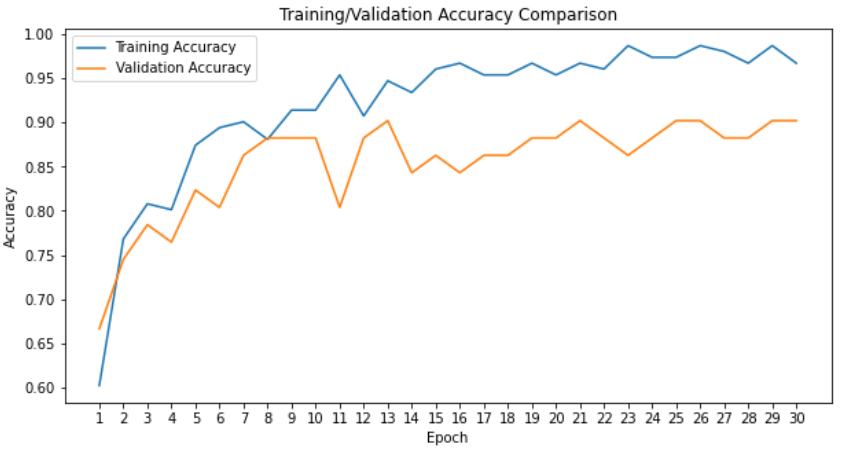
\includegraphics[width=3.5in]{transferl_epoch_val_accuracy.PNG}
    \caption{Transfer Learning Model Accuracy throughout the Epochs}\label{fig:fig16}
\end{figure}

\begin{figure}[H]
    \centering
    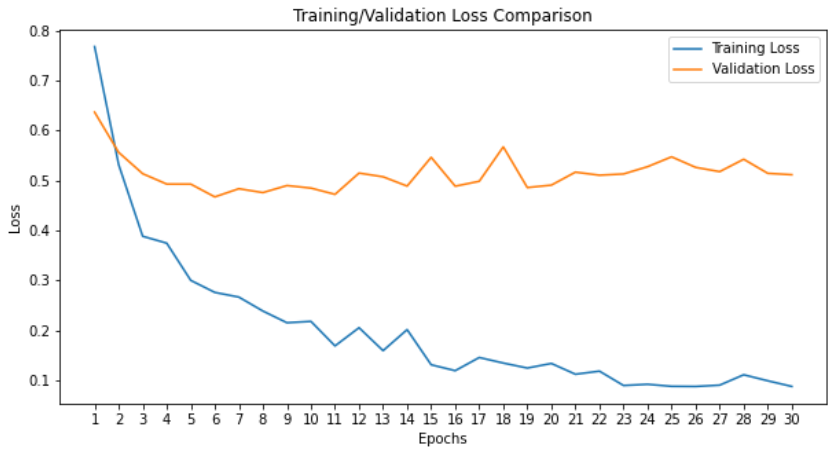
\includegraphics[width=3.5in]{transferl_epoch_val_loss.PNG}
    \caption{Transfer Learning Model Loss throughout the Epochs}\label{fig:fig17}
\end{figure}

\subsection{Learning Rate}

The learning rate is a hyper-parameter that controls how much the weights of the model change with the loss value throughout the epochs. According to this link\cite{b1}, a common way to select it is by validating the model with different powers of 10 between 0.000001 and 1. Using this approach to our deep learning models we were able to select the one that allowed for the best performance.

\subsubsection{CNN Model}
As shown in the graphs below, when comparing all the tested learning rates, the ones who were the most consistent were the ones that present a 0.001 learning rate, yet the difference present in the losses from each learning rate was not significant, excluding the value 0.1 which ends up converging towards the other loss functions.
\begin{figure}[H]
    \centering
    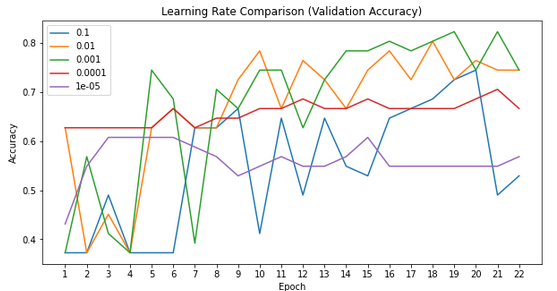
\includegraphics[width=3.5in]{learning_rates_cnn.png}
    \caption{CNN Model Accuracy Comparison with different learning rates}\label{fig:fig18}
\end{figure}

\begin{figure}[H]
    \centering
    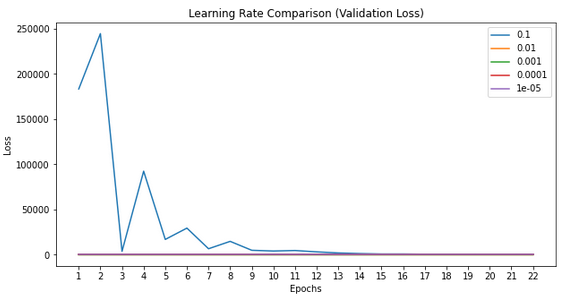
\includegraphics[width=3.5in]{loss_cnn.png}
    \caption{CNN Model Loss Comparison with different learning rates}\label{fig:fig19}
\end{figure}

\subsubsection{Transfer Learning Model}

According to the images below the best learning rate both in terms of validation accuracy and validation loss is 0.00001 and therefore it was chosen value for the learning rate of this model.

\begin{figure}[H]
    \centering
    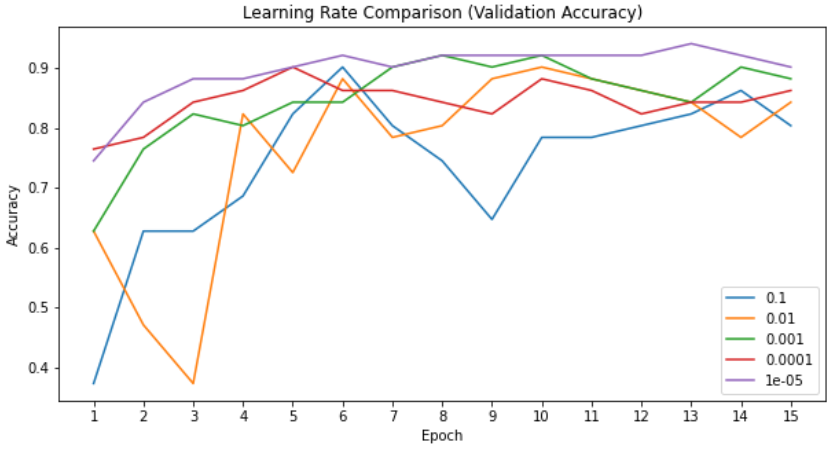
\includegraphics[width=3.5in]{transferl_learning_rate_val_accuracy.PNG}
    \caption{Transfer Learning Model Accuracy for different Learning Rates}\label{fig:fig20}
\end{figure}

\begin{figure}[H]
    \centering
    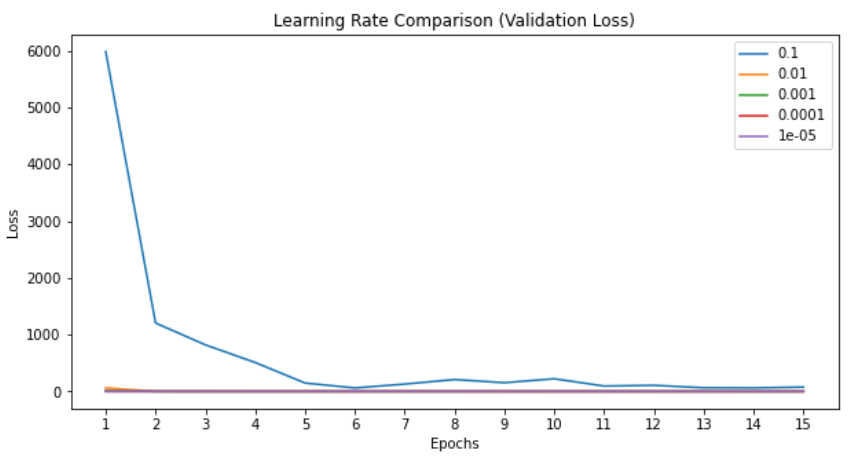
\includegraphics[width=3.5in]{transferl_learning_rate_val_loss.PNG}
    \caption{Transfer Learning Model Loss for different Learning Rates}\label{fig:fig21}
\end{figure}

\section{Model Comparison and Previous Work}

Among our models, the Transfer Learning Model has the best performance with 92\% accuracy.

Comparing our models with already existing work by other authors our models were unable to achieve a better performance in any type of model. Although we used similar architectures we tried to create our version of data augmentation which was unable to surpass the performance of the one that the library Keras has. Additionally, we also tried to innovate with techniques of undersampling and oversampling which were not in any project analyzed by us but they did not provide better results.

\section{Conclusion}

To conclude, this project contains the implementation of 3 models from 3 different types alongside the pre-processing of our chosen data set. Between all the models we obtained accuracies between 80\% and 92\%, with the Transfer Learning Model being the better performing one. Still, the results could be improved. For example, if we relied more on Keras to make our data augmentation we would be able to keep up with the previous work done on the dataset. Additionally, with more computation power we would be able to test increasing the image size or testing more complex models.

\begin{thebibliography}{00}
\bibitem{b1} Brownlee, J. (2019, August 6). How to Configure the Learning Rate When Training Deep Learning Neural Networks. Machine Learning Mastery. \url{https://machinelearningmastery.com/learning-rate-for-deep-learning-neural-networks/}.
\bibitem{b2} Brownlee, J. (2022). How to Configure Image Data Augmentation in Keras. Retrieved 4 May 2022, from \url{https://machinelearningmastery.com/how-to-configure-image-data-augmentation-when-training-deep-learning-neural-networks/}
\bibitem{b3} T. (2022, April 8). Brain Tumor Detection with Keras - 98\% accuracy. Kaggle. \url{https://www.kaggle.com/code/toobajamal/brain-tumor-detection-with-keras-98-accuracy}.
\bibitem{b4} Team, D. (2021, May 19). Brain Tumor Classification using Machine Learning. DataFlair. \url{https://data-flair.training/blogs/brain-tumor-classification-machine-learning/}.
\bibitem{b5} Pal, T. (2022, February 5). Brain Tumor Detection & Transfer Learning using VGG16. Medium. \url{https://medium.com/mlearning-ai/brain-tumor-detection-transfer-learning-using-vgg16-a0d0a31f2e9}.
\bibitem{b6} GeeksforGeeks. (2020, October 24). Intuition of Adam Optimizer. \url{https://www.geeksforgeeks.org/intuition-of-adam-optimizer/}.
\bibitem{b7} Baheti, P. (2022, March 19). The Train, Validation, and Test Sets: How to Split Your Machine Learning Data. V7. \url{https://www.v7labs.com/blog/train-validation-test-set}.
\bibitem{b8} Brain MRI Images for Brain Tumor Detection. (2019, April 14). Kaggle. \url{https://www.kaggle.com/datasets/navoneel/brain-mri-images-for-brain-tumor-detection/code}.
\bibitem{b9} Gandhi, R. (2018, July 5). Support Vector Machine — Introduction to Machine Learning Algorithms. Medium. \url{https://towardsdatascience.com/support-vector-machine-introduction-to-machine-learning-algorithms-934a444fca47}.
\bibitem{b10} Shanmukh, V. (2022, January 1). Image Classification Using Machine Learning-Support Vector Machine(SVM). Medium. \url{https://medium.com/analytics-vidhya/image-classification-using-machine-learning-support-vector-machine-svm-dc7a0ec92e01}.
\bibitem{b11} B. (2021, April 26). Brain MRI Tumor Detection using SVM. Kaggle. \url{https://www.kaggle.com/code/brendonim/brain-mri-tumor-detection-using-svm}.
\bibitem{b12} Gandhi, A. (2021, May 20). Data Augmentation | How to use Deep Learning when you have Limited Data. AI & Machine Learning Blog. \url{https://nanonets.com/blog/data-augmentation-how-to-use-deep-learning-when-you-have-limited-data-part-2/}.
\bibitem{b13} E. (2020, June 11). Brain Tumour Detection with CNN 96\% accuracy. Kaggle. \url{https://www.kaggle.com/code/ethernext/brain-tumour-detection-with-cnn-96-accuracy}.
\end{thebibliography}

\end{document}
